As we have just seen, concurrent (simultaneous) access of the shared data is a real performance killer. Intuitively, it makes sense: in order to avoid a data race, only one thread can operate on the shared data at any given time. We can accomplish this with a mutex or use an atomic operation if one is available. Either way, when one thread is, say, incrementing the shared variable, all other threads have to wait. Our measurements in the last section confirm it.

However, before taking any action based on observations and experiments, it is critically important to understand precisely what we measured and what can be concluded with certainty.

It is easy to describe what was observed: incrementing a shared variable from multiple threads at the same time does not scale at all and, in fact, is slower than using just one thread. This is true for both atomic shared variables and non-atomic variables guarded by mutex. We have not tried to measure unguarded access to a non-atomic variable because such an operation leads to undefined behavior and incorrect results. We also know that unguarded access to variables that are thread-specific (not shared) scales very well with the number of threads, at least until we saturate the aggregate memory bandwidth (which can only happen if we write large amounts of data; for a single variable this is not an issue). Analyzing your experimental results critically and without unjustified preconceptions is a very important skill, so let us state again what we know: guarded access to shared data is slow and unguarded access to non-shared data is fast. If we conclude from this that data sharing makes your program slow, we are making an assumption: shared data is what's important, guarded access is not. This brings up another very important point you should remember when doing performance measurements: when comparing two versions of the program, try to change only one thing at a time and measure the result.

The measurement we are missing is this one: non-shared access to guarded data. Of course, we don't really need to protect accesses to data that is accessed by only one thread, but we are trying to understand exactly what makes shared data access so expensive: the fact that it is shared or the fact that it is atomic (or protected by the lock). We have to make one change at a time, so let us keep the atomic access and remove data sharing. There are at least two simple ways to do this. The first one is to create a global array of atomic variables and have each thread access its own array element:

\begin{lstlisting}[style=styleCXX]
// 04_local_incr.C
std::atomic<unsigned long> a[1024];
void BM_false_shared(benchmark::State& state) {
	std::atomic<unsigned long>& x = a[state.thread_index];
	for (auto _ : state) {
		benchmark::DoNotOptimize(++x);
	}
}
\end{lstlisting}

The thread index in Google Benchmark is unique for each thread, the numbers start from 0 and are compact (0, 1, 2…). The other simple way is to declare the variable in the benchmark function itself as shown in the following code:

\begin{lstlisting}[style=styleCXX]
// 04_local_incr.C
void BM_not_shared(benchmark::State& state) {
	std::atomic<unsigned long> x;
	for (auto _ : state) {
		benchmark::DoNotOptimize(++x);
	}
}
\end{lstlisting}

Now we are incrementing the same atomic integer as we did when we collected the measurements for Figure 5.4, only it is no longer shared between threads. This will tell us whether it is the sharing or the atomic variable that makes the increment slow. Here are the results:

\hspace*{\fill} \\ %插入空行
\begin{center}
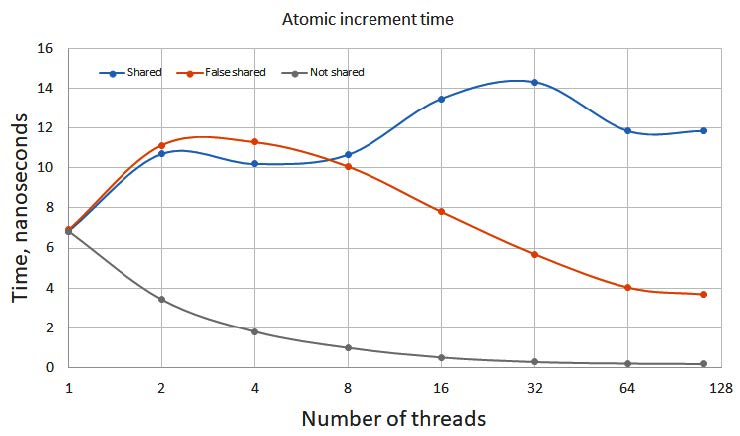
\includegraphics[width=0.9\textwidth]{content/1/chapter5/images/6.jpg}\\
Figure 5.6 – Atomic increment time for shared and not shared variables
\end{center}

The Shared curve is the one from Figure 5.4, while the other two are from the benchmarks without data sharing. The benchmark with a local variable on each thread is labeled Not shared and behaves as such: the computation on two threads takes half the time compared to that on one thread, going to four threads cuts the time by half again, and so on. Remember that this is the average time of one increment operation: we do, say, 1 million increments in total, measure the total time it takes, and divide by a million. Since the variables that we increment are not shared between threads, we expect two threads to run twice as fast as one thread, so the Not shared result is exactly what we expected. The other benchmark, the one where we use an array of atomic variables, but each thread uses its own array element, also has no shared data. However, it performs as if the data was shared between threads, at least for a small number of threads, so we call it False sharing: nothing is really shared, but the program behaves as if it was.

This result shows that the reason for the high cost of data sharing is more complex than what we assumed previously: in the case of false sharing, only one thread is operating on each array element, so it does not have to wait for any other thread to complete its increment. And yet, threads clearly wait for each other. To understand this anomaly, we have to learn more about the way caches work.

The way the data moves between the processors and the memory in a multi-core or a multi-processor system is illustrated in Figure 5.7.

\hspace*{\fill} \\ %插入空行
\begin{center}
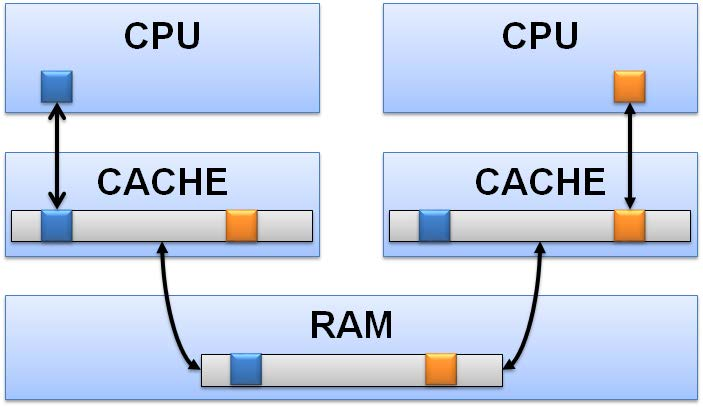
\includegraphics[width=0.9\textwidth]{content/1/chapter5/images/7.jpg}\\
Figure 5.7 – Data transfer between CPUs and memory in a multi-core system
\end{center}

The processor operates on the data in individual bytes, or in words that depend on the type of the variable; in our case, an unsigned long is an 8-byte word. An atomic increment reads a single word at the specified address, increments it, and writes it back. But reads from where? The CPU has direct access only to the L1 cache, so it gets the data from there. How does the data get from the main memory into the cache? It's copied over the memory bus, which is much wider. The minimum amount of data that can be copied from memory to cache and back is called a cache line. On all x86 CPUs, one cache line is 64 bytes. When a CPU needs to lock a memory location for an atomic transaction, such as an atomic increment, it may be writing a single word, but it has to lock the entire cache line: if two CPUs are allowed to write the same cache line into memory at the same time, one of them will overwrite the other. Note that, for simplicity, we show only one level of cache hierarchy in Figure 5.7, but it makes no difference: data travels through all cache levels in chunks of cache line length.

Now we can explain the false sharing we observed: even though the adjacent array elements are not really shared between threads, they do occupy the same cache line. When a CPU requests exclusive access to one array element for the duration of the atomic increment operation, it locks the entire cache line and prevents any other CPU from accessing any data in it. Incidentally, this explains why the false sharing in Figure 5.7 appears equivalent to the true data sharing for up to 8 threads but becomes faster for more threads: we are writing 8-byte words, so 8 of them fit into the same cache line. If we have only 8 threads (or fewer), only one thread can increment its value at any given time, the same as for true sharing. But with more than 8 threads, the array occupies at least two cache lines, and they can be locked by two CPUs independently from each other. So, if we have, say, 16 threads at any time, there are two threads that can move forward, one for each half of the array.

On the other hand, the real no-sharing benchmark allocates the atomic variables on the stack of each thread. These are completely independent memory allocations, separated by many cache lines. With no interaction through memory, these threads run completely independently of each other.

Our analysis shows that the real reason for the high cost of accessing the shared data is the work that must be done to maintain the exclusive access to a cache line and to make sure all CPUs have consistent data in their caches: after one CPU has obtained exclusive access and updated even one bit in the cache line, the copy of that line in all caches of all other CPUs is out of date. Before these other CPUs can access any data in the same cache line, they must fetch the updated content from the main memory, which, as we have seen, takes a relatively long time.

As we have seen, it doesn't really matter whether two threads try to access the same memory location or not, as long as they are competing for access to the same cache line. That exclusive cache line access is the origin of the high cost of shared variables. 

One may wonder whether the reason locks are expensive is also found in the shared data they contain (all locks must have some amount of shared data, that's the only way one thread can let another thread know that the lock is taken). A mutex lock is much more expensive than single atomic access, even on one thread, as we have seen in Figures 5.4 and 5.5. We can assume, correctly, that locking a mutex involves more work than just modifying one atomic variable. But why does this work take more time when we have more than one thread? Is it because the data is shared and needs exclusive access to the cache line? We leave it as an exercise to the reader to confirm that this is indeed so. The key to this experiment is to set up false sharing of locks: an array of locks such that each thread operates on its own lock, but they compete for the same cache line (of course, such per-thread locks don't actually protect anything from concurrent access, but all we want is the time it takes to lock and unlock them). The experiment is slightly more complex than you might think: the standard C++ mutex, std::mutex, is usually quite large, between 40 and 80 bytes depending on the OS. This means you can't fit even two of them into the same cache line. You have to do this experiment with a smaller lock, such as a spinlock or a futex.

We now understand why the cost of accessing the shared data concurrently is so high. This understanding gives us two important lessons. The first one is to avoid false data sharing when we attempt to create non-shared data. How can the unintended false sharing creep into our program? Consider the simple example we have studied throughout this chapter: accumulating a sum concurrently. Some of our approaches were slower than others, but they were all very slow (slower than the single-threaded program, or, at best, no faster). We understand that accessing shared data is expensive. So, what is less expensive? Not accessing the shared data, of course! Or at least not accessing it as often. There is no reason for us to access the shared sum value every time we want to add something to it: we can make all the additions locally, on the thread, and add them to the shared accumulator value once, at the very end. The code would look something like this: 

\begin{lstlisting}[style=styleCXX]
// 04_local_incr.C

// Global (shared) results
std::atomic<unsigned long> sum;
unsigned long local_sum[…];
// Per-thread work is done here
unsigned long& x = local_sum[thread_index];
for (size_t i = 0; i < N; ++i) ++x;
sum += x;
\end{lstlisting}

We have the global result, sum, that is shared between all threads and must be atomic (or protected by a lock). But each thread accesses this variable exactly once after all the work is done. Each thread uses another variable to hold the partial sum, only the values added on this thread (increments of 1 in our trivial case, but the performance is the same regardless of the values being added). We can create a large array to store these per-thread partial sums and give each thread a unique array element to work on. Of course, in this trivial example, we could just use a local variable, but in a real program, the partial results often need to be kept after the worker threads are done, and the final processing of these results is done elsewhere, perhaps by another thread. To simulate this kind of implementation, we use an array of per-thread variables. Note that these variables are just plain integers, not atomic: there is no concurrent access to them. Unfortunately, in the process, we fell into the trap of false sharing: the adjacent elements of the array are (usually) on the same cache line and, thus, cannot be accessed concurrently. This is reflected in the performance of our program:

\hspace*{\fill} \\ %插入空行
\begin{center}
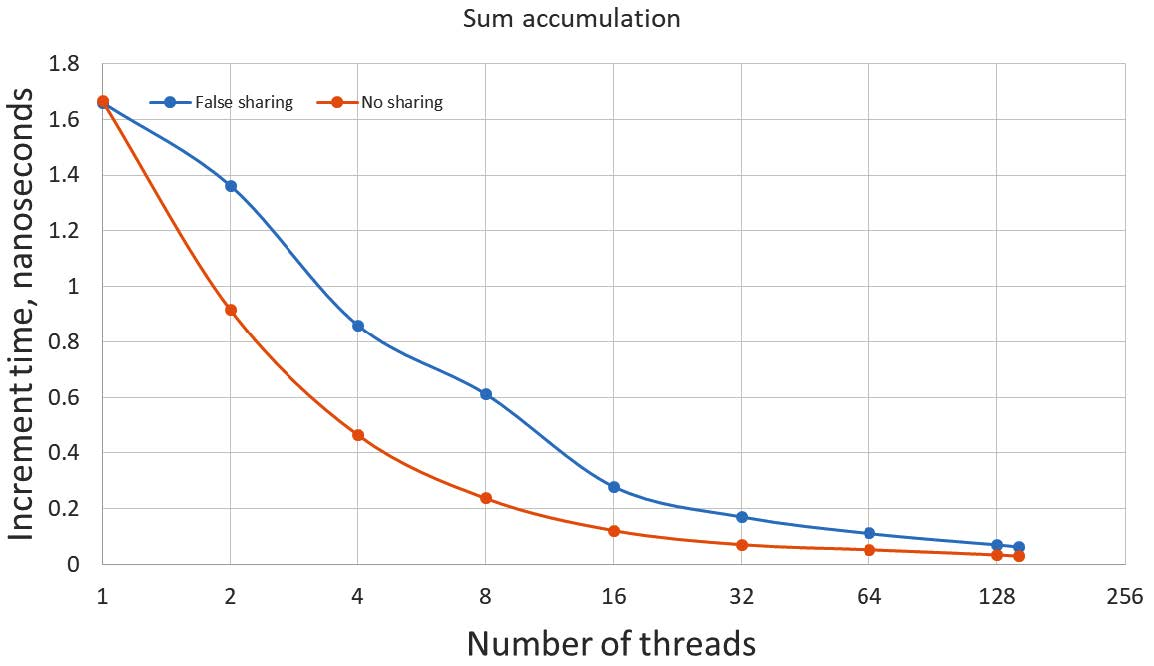
\includegraphics[width=0.9\textwidth]{content/1/chapter5/images/8.jpg}\\
Figure 5.8 – Sum accumulation with and without false sharing
\end{center}

As you can see in Figure 5.8, our program scales very poorly until we get to a very large number of threads. On the other hand, it scales perfectly, as expected, if we eliminate the false sharing by making sure the per-thread partial sums are at least 64 bytes apart (or simply using local variables in our case). While both programs become faster when we use more threads, the implementation that is not burdened by the false sharing remains approximately twice as fast.

The second lesson will become more important in the later chapters: since accessing shared variables concurrently is, comparatively, very expensive, an algorithm or an implementation that uses fewer shared variables will, in general, perform faster.

This statement may be confusing at the moment: by nature of the problem, we have some amount of the data that must be shared. We can do optimizations like the one we just did and eliminate unnecessary accesses to this data. But once this is done, the rest is the data we need to access to produce the desired results. How can there be more, or fewer, shared variables, then? To understand this, we have to realize that there is more to writing concurrent programs than protecting access to all shared data.






































